% version 1.01, date 07/03/16, auteur Matthieu Martins-Baltar
\documentclass[compress,xcolor=dvipsnames]{beamer}

%Pour les schémas d'architecture
\usepackage{etex}
\usepackage{tikz}
\usetikzlibrary{shapes,arrows,chains,backgrounds,fit}
%FIN Pour les shémas d'architecture

\usepackage[french]{babel}
\selectlanguage{french}
\usepackage[utf8]{inputenc}
\usepackage[T1]{fontenc}
\usepackage{tikz}
\usepackage{wrapfig}
\usepackage{multirow}
\usepackage{pgfplots}
\usepackage{pdfpages}
\usepackage{vocabulaireUnipikPresentation}
\usepackage{commun/vocabulaireCommun}
\usepackage{hyperref}
\usepackage{movie15}
\usepackage{xcolor}
\usepackage{lscape}
\usepackage{booktabs}
\usepackage{multirow}
\usepackage{colortbl}

\AtBeginSection[]{
  \begin{frame}
  \vfill
  \centering
  \begin{beamercolorbox}[sep=8pt,center,shadow=true,rounded=true]{title}
    \usebeamerfont{title}\insertsectionhead\par%
  \end{beamercolorbox}
  \vfill
  \end{frame}
}

\newcommand{\tabincell}[2]{\begin{tabular}{@{}#1@{}}#2\end{tabular}}

\usetheme{Berlin}%{Madrid}
\addtobeamertemplate{footline}{\hfill\insertframenumber/\inserttotalframenumber\hspace{2em}\null}
 
 
%Information to be included in the title page:
\title{Débriefing \CP}
\date{\today}
\author{\Sergi}
\institute{\insa}

\setbeameroption{show notes}

\begin{document}


\begin{frame}[plain]
	\titlepage
\end{frame}


\begin{frame}{Sommaire}
	\tableofcontents[hideallsubsections]
\end{frame}



\section[Gestion de l'équipe]{Gestion de l'équipe}
\subsection{}
\begin{frame}
\frametitle{Organigramme fonctionnel}
\begin{figure}
	\includegraphics[scale=0.15]{images/organigrammeFonctionnel.pdf}
	\caption{Organigramme fonctionnel}
	\label{OF}
\end{figure}
\end{frame}


\subsection{}
\begin{frame}
\frametitle{Gestion des compétences}
\begin{block}{Gestion des compétences}
\begin{itemize}
	\item Fiches de rôle
	\item Fiches de compétences
	\item Fiches de formation
	\item Fiches de suivi
	\item Observation continue
\end{itemize}
\end{block}
\end{frame}


\subsection{}
\begin{frame}
\frametitle{Méthodologie de travail}
\begin{figure}
\begin{center}
\includegraphics[scale=0.25]{images/modeleSpirale.pdf}
\caption{Modèle en spirale}
\label{MS}
\end{center}
\end{figure}
\end{frame}

\begin{frame}
\frametitle{Deux équipes de travail}
\begin{block}{Deux équipes}
\begin{itemize}
	\item Équipe Front-End
	\item Équipe Back-End
\end{itemize}
\end{block}
\end{frame}


\subsection{}
\begin{frame}
\frametitle{Communication interne}
\begin{block}{Différents moyens mis en place}
\begin{itemize}
	\item Réunions
	\item Open space
	\item Discord
	\item Boite à idée
\end{itemize}
\end{block}
\end{frame}


\subsection{}
\begin{frame}
\frametitle{Ambiance interne}
\begin{block}{Cohésion de groupe}
\begin{itemize}
	\item Team building
	\item Résolution de conflits
\end{itemize}
\end{block}
\end{frame}


\subsection{}
\begin{frame}
\frametitle{Animation des réunions}
\begin{block}{Animation des réunions}
\begin{itemize}
	\item Ordre du jour
	\item Expression libre
	\item Remarques
	\item Étude des risques et opportunités
\end{itemize}
\end{block}
\end{frame}



\section{Gestion du temps et des tâches}
\subsection{}
\begin{frame}
\frametitle{Planification des tâches}
\begin{figure}
\begin{center}
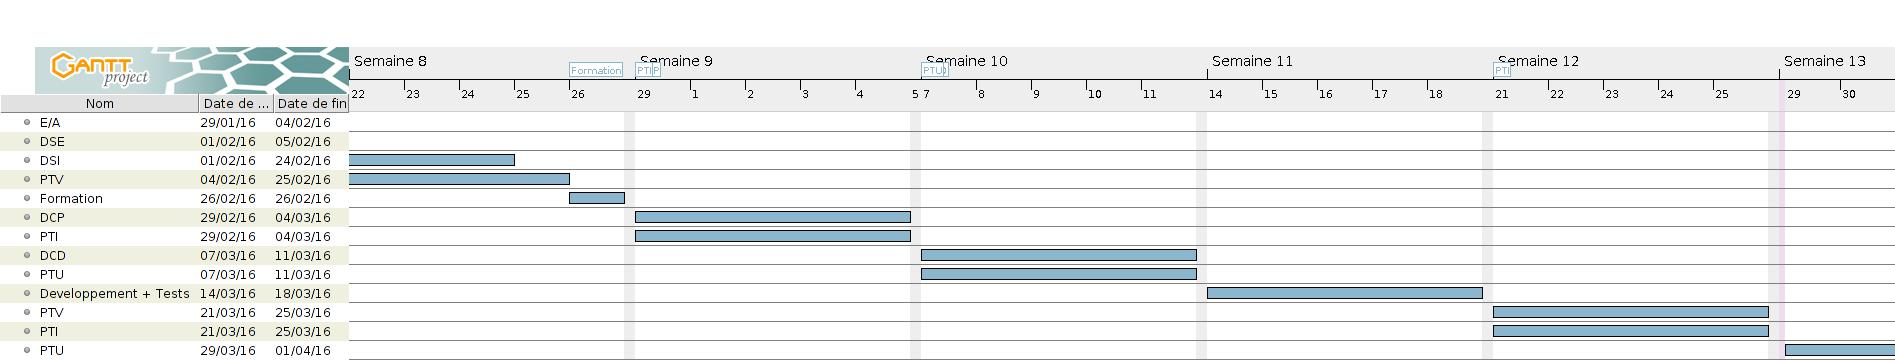
\includegraphics[scale=0.2]{images/exempleGantt.jpg}
\caption{Exemple de diagramme de Gantt}
\label{DG}
\end{center}
\end{figure}
\end{frame}

\begin{frame}
\frametitle{Planification des tâches}
\begin{figure}
\begin{center}
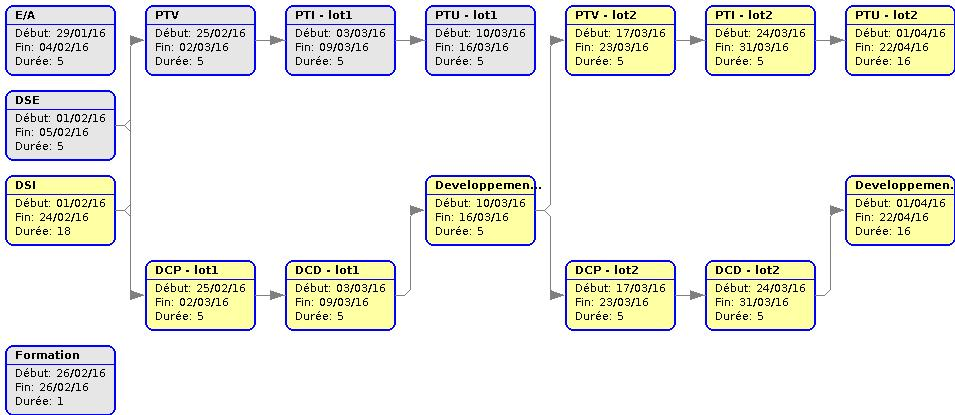
\includegraphics[scale=0.3]{images/exemplePert.jpg}
\caption{Exemple de diagramme de Pert}
\label{DP}
\end{center}
\end{figure}
\end{frame}


\subsection{}
\begin{frame}
\frametitle{Répartition des tâches}
\begin{block}{Trois possibilités}
\begin{itemize}
	\item Réunions
	\item Rôles
	\item Kanban
\end{itemize}
\end{block}
\end{frame}



\section{Relation client}
\subsection{}
\begin{frame}
\frametitle{Présentation du client}
\begin{block}{Rappel}
\begin{itemize}
	\item UNICEF 76
	\item Véronique Barbier
	\item Peu technique
	\item Association loi 1901
\end{itemize}
\end{block}
\end{frame}


\subsection{}
\begin{frame}
\frametitle{Communication Client}
\begin{block}{Relation avec le client}
\begin{itemize}
	\item Contact régulier
	\item Indisponibilités
	\item Reformulation
\end{itemize}
\end{block}
\end{frame}


\subsection{}
\begin{frame}
\frametitle{Partenariat}
\begin{block}{Partenariat INSA - UNICEF 76}
\begin{itemize}
	\item Hébergement par l'INSA
	\item UNICEF Campus
\end{itemize}
\end{block}
\end{frame}



\section{Qualité}
\subsection{}
\begin{frame}
\frametitle{Documents de qualité}
\begin{block}{Documents de qualité}
\begin{itemize}
	\item Aide à la rédaction
	\item Validation des documents
\end{itemize}
\end{block}
\end{frame}


\subsection{}
\begin{frame}
\frametitle{Faits techniques}
\begin{block}{Traitement des Faits Techniques}
\begin{itemize}
	\item Rédaction de FFT
	\item Correction de FT
	\item CTFT
\end{itemize}
\end{block}
\end{frame}


\subsection{}
\begin{frame}
\frametitle{Suivi des risques et opportunités}
\begin{block}{Risques et opportunités}
\begin{itemize}
	\item Étude hebdomadaire
	\item Analyse des risques et opportunités
	\item 16 risques
	\item 7 opportunités
\end{itemize}
\end{block}
\end{frame}



\section{Difficultés rencontrées}
\subsection{}
\begin{frame}
\frametitle{Retard livrable}
\begin{block}{Retard livraison}
\begin{itemize}
	\item Analyse des technologies utilisées
	\item Ajustement du planning
	\item Négociation client
\end{itemize}
\end{block}
\end{frame}


\subsection{}
\begin{frame}
\frametitle{Demande à la CNIL}
\begin{block}{Demande effectuée}
\begin{itemize}
	\item Manque d’expérience
	\item Collaboration avec le client et l'INSA
	\item Double déclaration
\end{itemize}
\end{block}
\end{frame}


\subsection{}
\begin{frame}
\frametitle{Demande d'hébergement}
\begin{block}{Personnes contactées}
\begin{itemize}
	\item Mme. Caldin
	\item M. Reynet
	\item M. Gasso
	\item Direction Générale
	\item M. Vasseur et M. Blondel-Angot
\end{itemize}
\end{block}
\end{frame}



\section{Conclusion}
\begin{frame}
\frametitle{Conclusion}
\begin{block}{Apport personnel}
\begin{itemize}
	\item Gestion de projet
	\item Communication avec un client
	\item Difficultés à surmonter
	\item Confiance en moi
\end{itemize}
\end{block}
\end{frame}

\end{document}
